\section{Scenarios}\label{sec:behaviourProblems}
In this section we will raise some questions that need attention or describe a situation where a behaviour needs to be defined for the system.

\textbf{Questions}
\begin{itemize}
\item When should a bicycle become unavailable for others, as a result of a booking?
\item When should a bicycle become available again after a booking has exceeded its reservation time?
\item How often does the GPS needs to read data?
\end{itemize}

\begin{description}[style=nextline]
\item[Problem 1.1] Consider the scenario where a user $u_1$ makes a booking $b_1$ on the website at time $t_1$ wanting to reserve a bicycle for time $t_3$. Before time $t_1$ another user $u_2$ made a booking $b_2$ of a bicycle for time $t_2$. Both users made a booking at the same station, and the amount of available bicycles for that station was for both users 1. Under the assumption that a bicycle cannot be locked and thereby reserved before some amount of time, say $t_{before}$, before usage, this scenario is possible in the following way.

First consider this definition of a time $t$, it is a time represented as the number of seconds from Thursday, 1 January 1970 at 00:00:00 UTC, which is the Epoch time, as of such comparisons such as $>$ is just computed as usual on numbers.
Let, 
$$TSB(b) = \{(t_1,t_2) | t_1 = st(b) - t_{before} \land t_2 = st(b) \land t_1 \leq t_2 \}$$
where,
\begin{itemize}[align = left]
	\item[$st(b)$] is defined as the start time of booking $b$.
	\item[$TSB(b)$] defines the Time Span Before of booking $b$.
\end{itemize} 

Then the scenario is given if $TSB(b_1) > TSB(b_2) > t_1$, where comparison of each time span $(t_1, t_2)$ is a comparison on the first element (e.g. $(t_1, t_2) > (t_3, t_4)$ if $t1 > t3$), and for comparison of a timespan to a time is comparison of the start-time of the timespan and the time.

The problem for user $u_1$ is then at time $t_1$ it appeared that a bicycle was available, but the bicycle will be locked for user $u_2$ (although not entirely certain, see Problem 1.2) before it will be locked for $u_1$ resulting in an availability count of 0 for $u_1$, thereby having no bicycle to lock for $u_1$.

\item[Problem 1.2] Having a booking system that is capable of capturing the state of each station, giving available bicycles and available free docks, along with the ability to borrow a bicycle without interacting with the booking system, imposes an element of unpredictability.

Given the scenario where a user reads the state of a station and make a booking $b$ on that station at a time $(t,t) < TSB(b)$ there is no certainty that a bicycle will be available to lock in $TSB(b)$, because other user may have borrowed the rest of the bicycles at that station before $TSB(b)$.

\item[Problem 1.3]
\begin{figure}
	\centering
	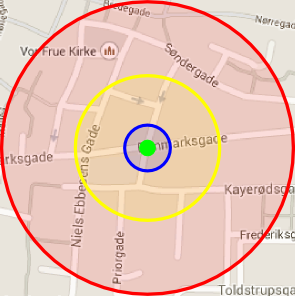
\includegraphics[scale=1]{GPScircles}
	\caption{Distance coverage with 20 km/h.}
	\label{fig:gpsCircles}
\end{figure}
\end{description}

\fxwarning{Forstår det ikke, fungerer systemet sådan som det antager? Falder antal tilgængelig cykler ikke når man laver en booking?}